\documentclass{beamer}
\usepackage[spanish]{babel}
\usepackage[utf8]{inputenc}
\usepackage{graphicx}
\usepackage{dcolumn}                                                                                                                                                                                              
\usepackage{datatool}

\usecolortheme[RGB={122,59,122}]{structure}

\newtheorem{definicion}{Definición}
\newtheorem{ejemplo}{Ejemplo}

\title{Integración Trapecio \\ $f(x)=sen(\Pi x)$, $x \in [-2,-1]$}
<<<<<<< HEAD
\author{Lára Kristjánsdóttir, Javier Hernández Pérez}
=======
\author{Lara Kristjansdottir, Javier Hernández Pérez\\ Técnicas Experimentales \\ Grupo 2F}
>>>>>>> d96aa33c5d0828c53f4262ea40320b64e7037390
\date{\today}
\usetheme{Madrid}
\begin{document}
\begin{frame}
  
\includegraphics[width=0.15\textwidth]{img/ullesc.eps}
  \hspace*{7.5cm}
  
\includegraphics[width=0.16\textwidth]{img/fmatesc.eps}
  \titlepage
  \begin{scriptsize}
    \begin{center}
    \title{Integración Trapecio de $f(x)=sen(\Pi x)$, $x \in [-2,-1]$}
      Facultad de Matemáticas \\Universidad de a Laguna
    \end{center}
  \end{scriptsize}
\end{frame}
%++++++++++++++++++++++++++++++++++++++++++++++++++++++++++++++++++++++++++++++++++++
%++++++++++++++++++++++++++++++++++++++++++++++++++++++++++++++++++++++++++++++++++++
\begin{frame}
  \frametitle{Contenido}
  \tableofcontents
\end{frame} 
%++++++++++++++++++++++++++++++++++++++++++++++++++++++++++++++++++++++++++++++++++++
%++++++++++++++++++++++++++++++++++++++++++++++++++++++++++++++++++++++++++++++++++++
\section{Motivación y objetivos}
\begin{frame}
\frametitle{Motivación}
%\begin{example}
\begin{enumerate}
\item El método de los trapecios y un terreno.\\
\pause
%\end {example}
\item La integral es fácil de resolver:\\
$\int _{-2}^{-1} sen(\pi x) dx=\frac{\int _{-2 \pi}^{-1\pi}sen(y)dy}{\pi}=\frac{-cos(-\pi)+cos(-2 \cdot \pi)}{\pi}=\frac{1+1}{\pi}=\frac{2}{\pi}\simeq 0,6366197724$
\end{enumerate}
\end{frame}

%++++++++++++++++++++++++++++++++++++++++++++++++++++++++++++++++++++++++++++++++++++
%++++++++++++++++++++++++++++++++++++++++++++++++++++++++++++++++++++++++++++++++++++
\section{Convergencia del método de los trapecios}
\begin{frame}
\begin {theorem}
Sea $f$:$[a,b]$ $\rightarrow$ $\mathbb{R}$ una función integrable en el intervalo cerrado $[a,b]$. Si $P=\{x_0,x_1,x_2,...,x_n\}$ es la partición de $[a,b]$ que divide a este intervalo en n partes iguales, entonces el siguiente número aproxima a la integral $\int_a^bf(x)dx$.

$I_t= \frac{b-a}{n}\left( \frac{f(a)}{2} + f(x_1)+f(x_2)+f(x_3)+...+f(x_{n-1})+\frac{f(b)} {2} \right)$

La aproximación tiene un error de si la función $f$ es $C^2$ y K es cota superior de la derivada segunda.

$|I_t-\int_a^bf(x)dx|\leq |\frac {(b-a)^3} {12n^2} K|$
\end {theorem}
\end{frame}
%++++++++++++++++++++++++++++++++++++++++++++++++++++++++++++++++++++++++++++++++++++
\begin {frame}
Demostración:\\
$F_\alpha :[0,h]\rightarrow \mathbb{R}$\\
$t\rightarrow F_\alpha(t)=\frac{t}{2} \left(f(\alpha)+f(\alpha+t) \right)-\int_\alpha ^{\alpha+t} f dt$\\
\pause
Derivando:\\
$F'_\alpha(t)=\frac{1}{2}\left(f(\alpha)+f(\alpha+t) \right) +\frac{t}{2} 0 + \frac{t}{2} f'(\alpha+t)  -f(\alpha+t) +0=\frac{1}{2}\left(f(\alpha)+f(\alpha+t) \right)+ \frac{t}{2} f'(\alpha+t)  -f(\alpha+t)=\frac {1}{2} \left(f(\alpha)-f(\alpha+t) \right)+ \frac{t}{2} f'(\alpha+t)$\\
\pause

$F''_\alpha(t)=\frac {1}{2} \left(0-f'(\alpha+t) \right)+ \frac{1}{2} f'(\alpha+t)+\frac{t}{2}f''(\alpha+t)=-\frac {1}{2} f'(\alpha+t) + \frac{1}{2} f'(\alpha+t)+\frac{t}{2}f''(\alpha+t)=\frac{t}{2}f''(\alpha+t)$\\

\end{frame}
%++++++++++++++++++++++++++++++++++++++++++++++++++++++++++++++++++++++++++++++++++++
\begin {frame}
K cota derivada segunda:\\
$|F''_\alpha(t)| \leq |\frac{t}{2} K|$
\pause
Integramos sabiendo $F'_\alpha(0)=\frac {1}{2} \left(f(\alpha)-f(\alpha+0) \right)+ \frac{0}{2} f'(\alpha+0)=0+0=0$\\
\pause
$|\int_0^t F''_\alpha(t)| \leq |\int_0^t\frac{t}{2} K| \Rightarrow |F'_\alpha(t)-F'_\alpha(0)| \leq |\frac{t^2}{4} K-\frac{0^2}{4} K| \Rightarrow |F'_\alpha(t)| \leq |\frac{t^2}{4} K|$
\pause
Además sabiendo
$F_\alpha(0)=\frac{0}{2} \left(f(\alpha)+f(\alpha+0) \right)-\int_\alpha ^{\alpha+0} f dt=0-0=0$ seguimos integrando\\

$|\int_0^h F'_\alpha(t)|\leq|\int_0^h \frac{t^2}{4} K| \Rightarrow |F_\alpha(h)-F_\alpha(0)| \leq |\frac{h^3}{12} K|-\frac{0^3}{12} K|\Rightarrow |F_\alpha(h)| \leq |\frac{h^3}{12} K|$
\pause
Haciéndolo en los n intervalos y sustituyendo h por su valor obtenemos la cota.\\

$|\frac{(b-a)^3}{12 (n^2)} K|$
\end{frame}
% *************************************************************************************
\section{Descripción de los experimentos}
\begin{frame}
  \frametitle{Descripción}
  Vamos a aplicar la regla del trapecio a la función sin(pi*x) en el intervalo [-2,-1] utilizando una cantidad variable de subintervalos, n. Para cada valor de n, mediremos el error absoluto y el tiempo de ejecución del método.
\end{frame}

\section{Resultados obtenidos}
\begin{frame}
  \frametitle{Resultados}
  
\DTLloaddb[noheader,keys={n,error,tiempo}]{table1}{mydata.csv}
\newcolumntype{d}{D{,}{\pm}{-1}} 

\begin{table}[!h]
 \begin{center}
  \begin{tabular}{l|c|r}% 
    {\bf n} & {\bf error} & {\bf tiempo}
    \DTLforeach*{table1}{%
      \n=n,\error=error,\tiempo=tiempo}{%
      \\
      \n & \error & \tiempo}%
  \end{tabular}
  \caption{Resultados optenidos por número de trapecios}
  \label{tabla:1}
  \end{center}
\end{table}                                     

\end{frame}

\begin{frame}
  \frametitle{Resultados}
  \begin{figure}[!th]
    \begin{center}
      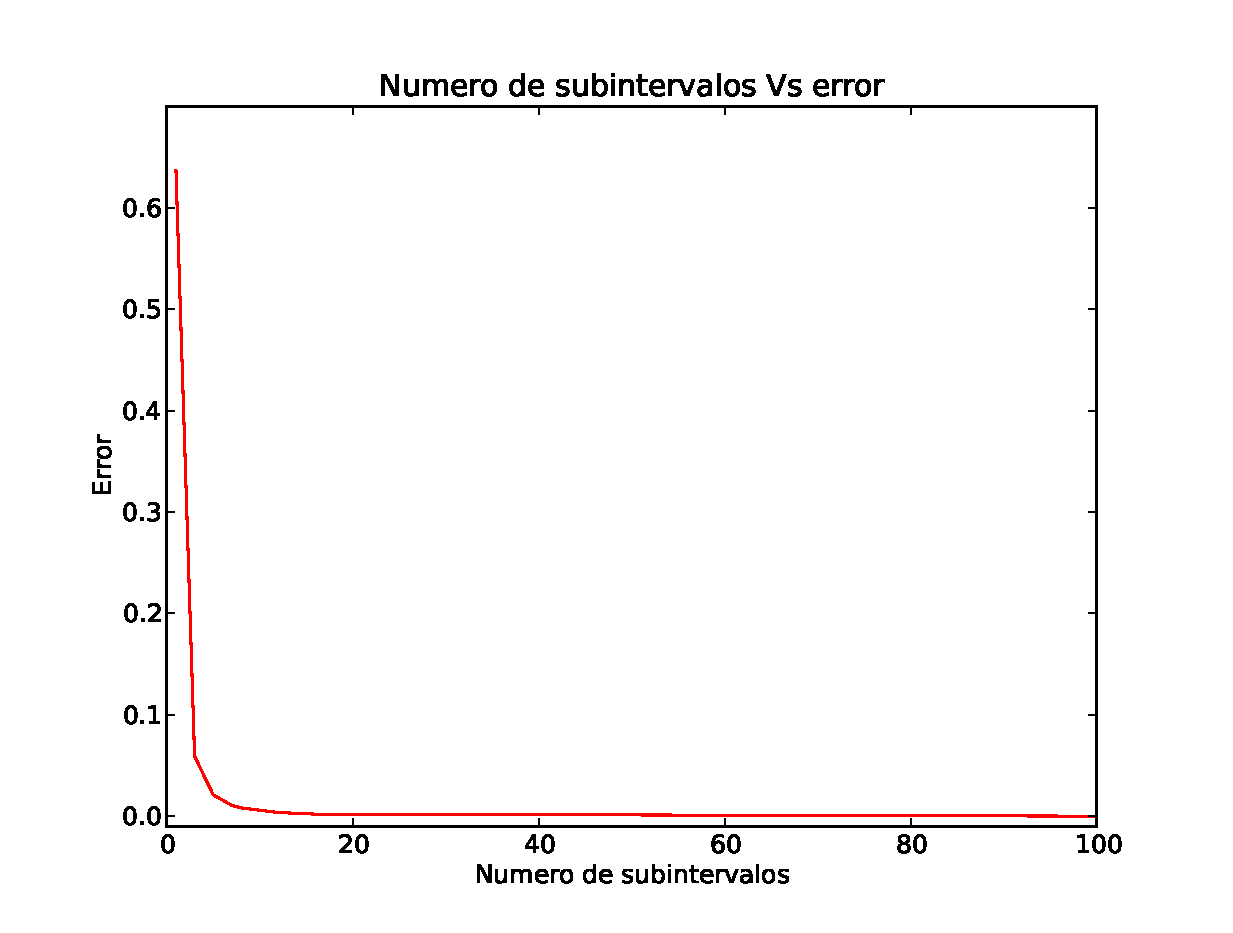
\includegraphics[width=0.75\textwidth]{img/Plot_nVSerror.eps}
      \caption{nVSerror}
      \label{fig:1}
    \end{center}
  \end{figure}
\end{frame}

\begin{frame}
  \frametitle{Resultados}
  \begin{figure}[!th]
    \begin{center}
      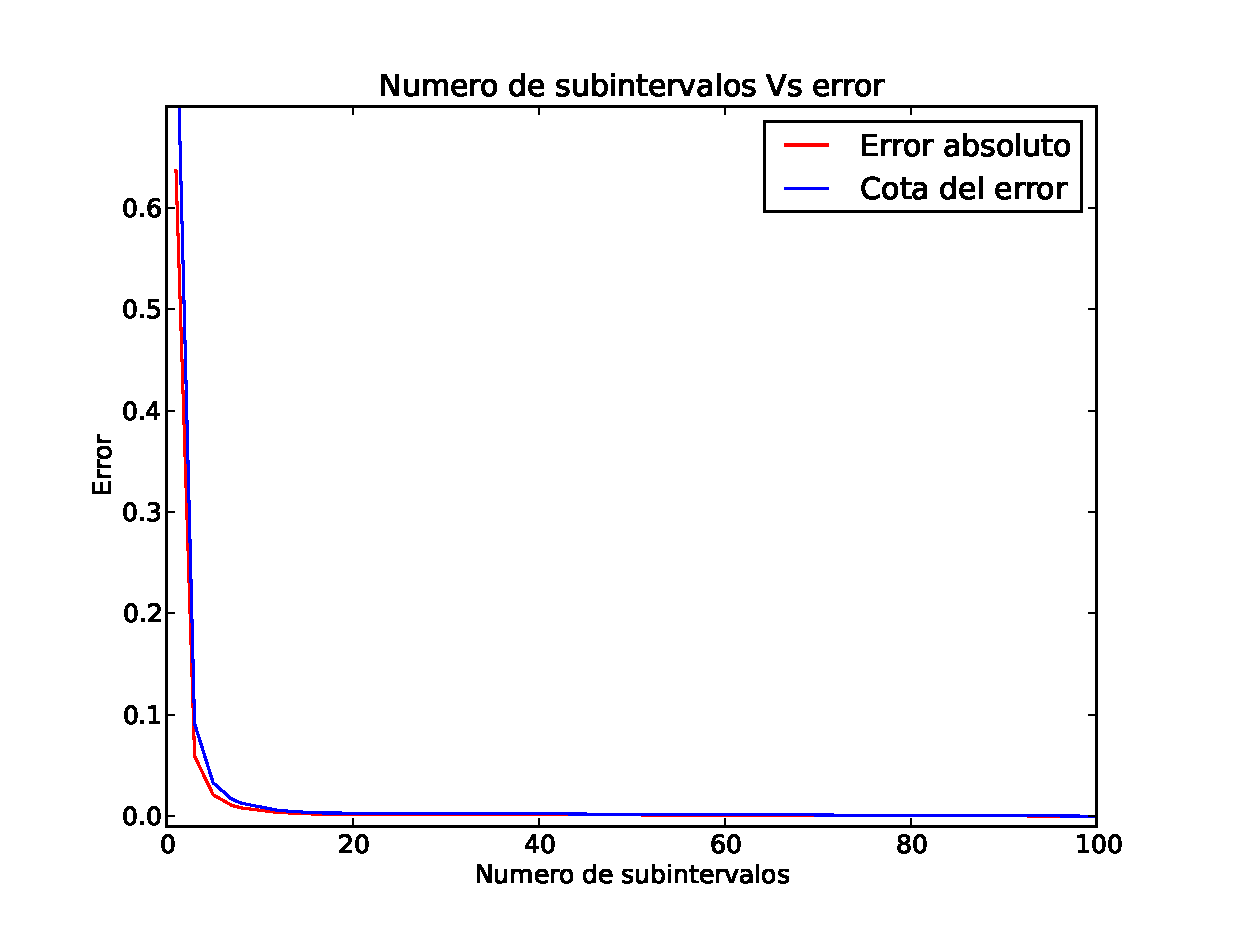
\includegraphics[width=0.75\textwidth]{img/Plot_nVSerrorAndcota.eps}
      \caption{nVSerror}
      \label{fig:1}
    \end{center}
  \end{figure}
\end{frame}

\begin{frame}
  \frametitle{Resultados}
  \begin{figure}[!th]
    \begin{center}
      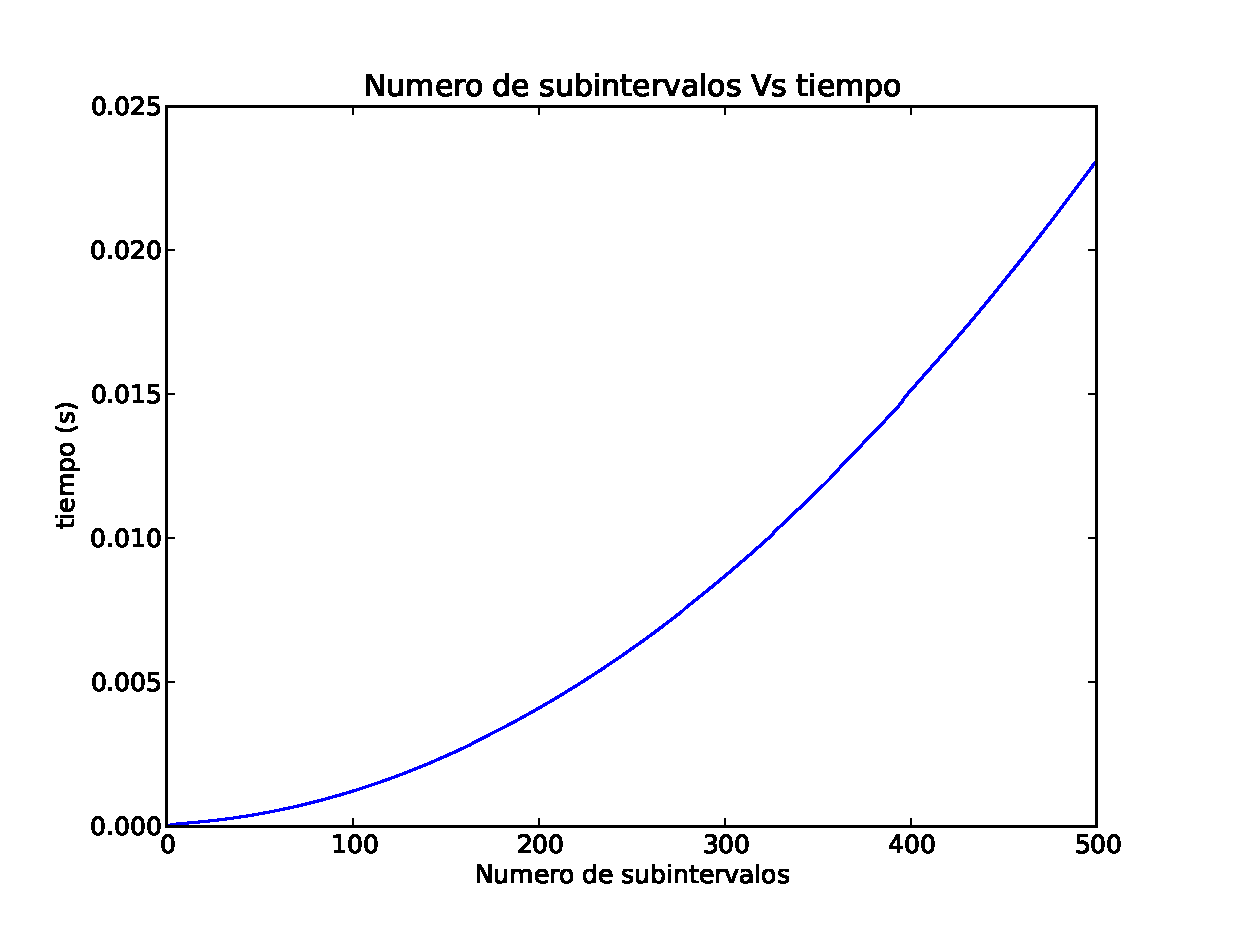
\includegraphics[width=0.75\textwidth]{img/Plot_nVStime.eps}
      \caption{nVStiempo}
      \label{fig:2}
    \end{center}
  \end{figure}
\end{frame}

\section{Concluciones}
\begin{frame}
 \frametitle{Concluciones}
\end{frame}



%++++++++++++++++++++++++++++++++++++++++++++++++++++++++++++++++++++++++++++++  
\begin{frame}
  \frametitle{Bibliografía}

  \begin{thebibliography}{10}

    \beamertemplatebookbibitems
    \bibitem[libro]{libro}  
    Juan de Burgos Román (2007) Cálculo infinitesimal de una variable segunda edición McGraw Hill
    
    \beamertemplatebookbibitems
    \bibitem[\LaTeX]{latex}  
    http://www.latex-project.org/
    
    \beamertemplatebookbibitems
    \bibitem[Python]{python}  
    http://www.python.org/
    
      
    
      \end{thebibliography}
\end{frame}


%++++++++++++++++++++++++++++++++++++++++++++++++++++++++++++++++++++++++++++++  

\end{document}